\scanpage{2}\mspage{1}
\margin{\handwritten{9/74\\ Envoyé par Grothendieck}}

\begin{center}
Esqu\deleted{ç}isse d'une théorie des Gr-Catégories\\
par Mme Hoang Xuan Sinh
\end{center}

Nous donnons un résumé de quelques résultats sur les (Gr)-catégories, faisant l'objet d'un travail détaillé que l'auteur compte présenter prochainement comme thèse de doctorat\handwritten{[\, ]}.

1. Structure des (Gr)-catégories.

Notre terminologie est celle de Saavedra \handwritten{[\, ]}. Nous nous intéressons à des catégories $C$ munies d'une opération binaire $(\deleted{x}X,Y)\handwritten{\mapsto}X\otimes Y$ (fonc\deleted{\rlap{xxx}\unsure{teu|te}}teur de $C\mathbin{\mathrm{x}}C$ dans $C$) associative et unitaire à isomorphisme donné près (satisfaisant des conditions de compatibilité explicitées dans loc. cit.), appelées aussi $\otimes$-catégories AU (associatives-unitaires). On dit qu'une telle catégorie est une (Gr)-catégorie si \inserted{\handwritten{c'est un groupoïde, et si}} tout objet $X$ de $C$ est ``inversible'', i.e. admet un objet ``inverse'' $Y=X^{-1}$ (satisfaisant $X\otimes Y\handwritten{\simeq}Y\otimes X\handwritten{\simeq}1_C$, où $1_C$ désigne l'objet unité de $C$). Les exemples abondent:

\uline{Exemple\unsure{\handwritten{s}|\deleted{s}}\unsure{.|,}\deleted{1}} \handwritten{1.} $X$ étant un espace topologique\inserted{ ponctué par $x\handwritten{\in}X$}, on prend pour $C$ la catégorie des lace\deleted{\rlap{x}\unsure{s|t}}ts de $X$ en $x$, avec comme morphismes les classes d'homotopie d'homotopies entre lacets, comme opération $\otimes$ la composition des lacets (qui n'est pas associative, mais associative ``à homotopie près'').
% Marginal reference arrow points up and right toward the line beginning pie d'homotopies.
\margin{\handwritten{\figure{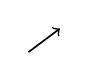
\begin{tikzpicture}[x=1cm,y=1cm]\draw[->,line width=.6pt] (0,0)--(.4,.3);\end{tikzpicture}}\unsure{Cet|cet} exemple \unsure{est|st} un cas \unsure{particulier} du \unsure{suivant}, en \unsure{prenant} $G$ $\unsure{\phantom{=}|=}\Omega^{1}(X,x)$ \unsure{(espace} des \unsure{lacets}).}}

% The recurring typed space symbol is overstruck; G is preferred, without asserting a special alphabet.
Variante: $\unsure{G|\mathbb{G}|E|K}$ est un espace de Hopf associatif (ou simplement homotopiquement associatif en un sens suffisamment fort), $C$ la catégorie dont les objets sont les points de $G$, les morphismes les classes d'homotopies de chemins entre points de $G$, la loi $\otimes$ étant induite par la loi de composition de $G$. (NB Lorsque $G$ admet un espace classifiant $X$, on retrouve essentiellement l'exemple précédent\handwritten{.)}\deleted{\handwritten{qui lui \unsure{même|mêmes} \illegible{2}}}

\deleted{\uline{Exemple}} 2. Si $F$ est un faisceau sur un espace topologique (ou plus généralement sur un topos), la catégorie $C$ des torseurs sous $F$, munie de la composition de Baer, est une (Gr)-catégorie (et même une catégorie de Picard stricte, cf. plus bas). On peut considérer la catégorie $C$ des Modules inversibles sur un espace (ou topos) \inserted{\handwritten{localement}} annelé \deleted{\rlap{xxxxx}comme} $(X,\underline{O}_{X})$ comme le cas particulier correspondant au cas $F=\underline{O}_{X}^{\handwritten{*}}$.

\deleted{\uline{Exemple}} 3. Si $A$ est une catégorie, la sous-catégorie pleine \inserted{\handwritten{$C$}} de $\underline{\mathrm{Hom}}(A,A)_{\handwritten{\mathrm{is}}}$ formée des équivalences de $A$ avec elle-même, munie de l\deleted{o}'opération de composition des foncteurs, est une (Gr)-catégorie. Au lieu de prendre pour $A$ une catégorie, on peut \inserted{\handwritten{plus généralement}} prendre pour $A$ un objet d'une 2-catégorie quelconque. Si p.ex. $F$ est un faisceau en groupes (pas nécessairement commutatif\deleted{\unsure{s|x}}) sur un espace topologique \handwritten{(}ou un topos\handwritten{)}\deleted{$X$}\handwritten{,}
% archive sheet number: 1
